\section{Subjective experiment}
We conducted a large-scale subjective experiment to evaluate the visual impact of texture and geometry distortions on the appearance of textured 3D models. We chose a paired comparisons technique, where observers are shown two stimulus side by side and are asked to choose the one that is most similar to the reference (forced-choice methodology). This protocol was shown to be more accurate than others (e.g. single stimulus rating) due to the simplicity of the subjects’ task \cite{Mantiuk2012}. This section details the subjective study and its results.

\subsection{Stimuli Generation}
We selected 5 textured triangle meshes created using different methodologies and targeting different application domains (see figure \ref{fig-ref}). The \textit{Hulk} and \textit{Sport Car} are artificial models created using a modeling software. They have been selected from a community model repository (ShareGC.com). They both have small numbers of polygons, structured texture content and smooth texture seams (i.e. vertices associated with multiple texture coordinate pairs). The \textit{squirrel} and the \textit{Easter Island statue} come from a reconstruction process using multiple photographs, they are courtesy of the EPFL Computer Graphics and Geometry Laboratory. Finally, the \textit{Dwarf} is a scanned model, courtesy of the Visual Computing Laboratory of ISTI-CNR, Pisa (http://vcg.isti.cnr.it). These three latter models, created respectively from reconstruction and scanning, exhibit noisier texture seams and content. Note that the \textit{Hulk} and \textit{Sport Car} are associated to several texture images (resp. 2 and 15). The numbers of vertices from the five models goes from 6,000 to 250,000 and the texture size goes from $256\times256$ (when several texture maps are used) to $4096\times4096$.  To summarize, these objects span a wide variety of geometry and texture data.\\
\begin{figure}
  \centering
  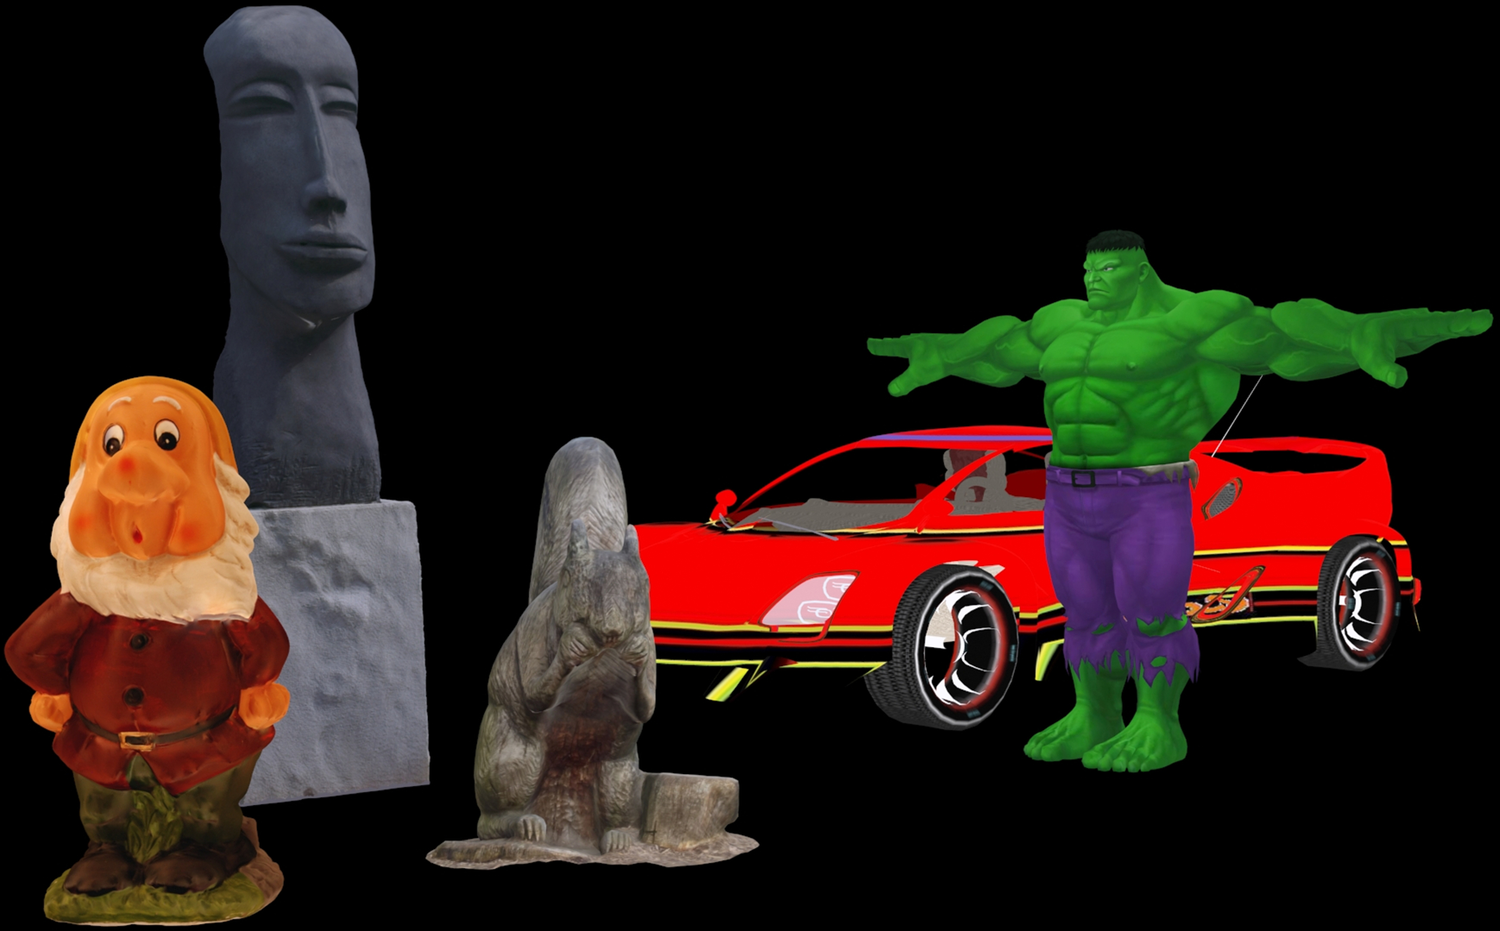
\includegraphics[width=.7\linewidth]{allmodels.png}
  \caption{\label{fig-ref} 5 Models used in the subjective study (from left to right: Dwarf, Easter Island statue, squirrel, Sport Car and Hulk)..}
  \end{figure}
These reference models have been corrupted by five types of distortions (three applied on the geometry and two applied on the texture), applied each with four different strengths:\\
On the geometry:
\begin{itemize}
\item \textbf{Compression} - We consider uniform geometric quantization, the most common lossy process of compression algorithms.
\item  \textbf{Simplification} - We consider the \textit{Quadric Error Metric} algorithm from \citet{GARLAND-1997}.
\item \textbf{Smoothing}: We consider Laplacian smoothing \cite{Taubin:1995}.
\end{itemize}
On the texture map:
\begin{itemize}
\item \textbf{JPEG}: The most commonly used algorithm for the lossy compression for 2D images.
\item \textbf{Sub-sampling}: We reduce the texture size by resampling through bilinear interpolation.
\end{itemize}
The strength of these distortions have been adjusted manually in order to span the whole range of visual quality from imperceptible levels to high levels of impairment. For this task, a large set of distortions were generated and viewed by the authors and a subset of them that spanned the desired visual quality (i.e. “Excellent”, “Good”, “Fair” and “Poor”) were chosen to be included in the database. This perceptual adjustment of the distortion strength was also done for the LIVE Video Quality Database \cite{Seshadrinathan2010}. As stated by the authors, it allows to test the ability of objective metrics to predict visual quality consistently across varying content and distortion types. We thus generated 20 distorted models (5 distortion types $\times$ 4 strength) per reference object. \\
To challenge the generalization ability of the objective metrics, we also included mixed distortions. For this task, we manually selected 36 distorted versions among the $12\times8=96$ possible combinations of the 12 geometry and 8 texture distortions detailed above. In practice we applied the 20 single-type distortions on the \textit{Hulk}, \textit{Sport Car}, \textit{squirrel} and \textit{Easter Island statue} model, and the mixed 36 mixed distortions on the \textit{Dwarf} model, resulting in a database of 116 models (+5 references), including the reference. Table \ref{tab-dis} details the distortion parameters while figure \ref{fig-dist} illustrate some visual examples.\\
\begin{table}[]
\centering
\caption{All the distortions applied on our models for the study}
\label{my-label}
\begin{tabular}{lllllll}
\textbf{ID} & \textbf{Distortion type} & \textbf{Method\&ref}        & \textbf{Squirral }      & \textbf{Hulk }        & \textbf{Easter Island statue} & \textbf{Sport Car }    \\
                &                        & Settings       & Settings     & Settings             & Settings       \\
\textit{L1} & Smoothing       & Taubin              & 1 iteration    & 1 iteration  & 10 iterations        & 1 iteration    \\
\textit{L2} & Smoothing       & Taubin              & 3 iterations   & 2 iterations & 20 iterations        & 3 iterations   \\
\textit{L3} & Smoothing       & Taubin              & 5 iterations   & 3 iterations & 30 iterations        & 5 iterations   \\
\textit{L4} & Smoothing       & Taubin              & 7 iterations   & 4 iterations & 50 iterations        & 7 iterations   \\
\textit{Si4} & Simplification  & Garland\&Eckbert \cite{Garland_1997}       & 87.5\% removed & 70\% removed & 95\% removed         & 87.5\% removed \\
\textit{Si3} & Simplification  & Garland\&Eckbert \cite{Garland_1997}       & 75\% removed   & 50\% removed & 87.5\% removed       & 75\% removed   \\
\textit{Si2} & Simplification  & Garland\&Eckbert \cite{Garland_1997}        & 70\% removed   & 40\% removed & 70\% removed         & 60\% removed   \\
\textit{Si1} & Simplification  & Garland\&Eckbert \cite{Garland_1997}       & 50\% removed   & 30\% removed & 50\% removed         & 50\% removed   \\
\textit{Q1 }& Quantization    & Uniform                & 7 bits         & 7 bits       & 7 bits               & 7 bits         \\
\textit{Q2} & Quantization    & Uniform                & 8 bits         & 8 bits       & 8 bits               & 8 bits         \\
\textit{Q3} & Quantization    & Uniform                & 9 bits         & 9 bits       & 9 bits               & 9 bits         \\
\textit{Q4} & Quantization    & Uniform                & 10 bits        & 10 bits      & 10 bits              & 10 bits        \\
\textit{J4} & JPEG            & DCT                    & 6\% quality    & 8\% quality  & 8\% quality          & 1\% quality    \\
\textit{J3} & JPEG            & DCT                    & 10\% quality   & 10\% quality & 12\% quality         & 3\% quality    \\
\textit{J2} & JPEG            & DCT                    & 14\% quality   & 14\% quality & 16\% quality         & 5\% quality    \\
\textit{J1} & JPEG            & DCT                    & 18\% quality   & 18\% quality & 80\% quality         & 10\% quality   \\
\textit{Su4} & Sub-sampling    & bilinear interpolation & 10\% sampled   & 10\% sampled & 5\% sampled          & 5\% sampled    \\
\textit{Su3} & Sub-sampling    & bilinear interpolation & 20\% sampled   & 20\% sampled & 10\% sampled         & 10\% sampled   \\
\textit{Su2} & Sub-sampling    & bilinear interpolation & 30\% sampled   & 30\% sampled & 20\% sampled         & 20\% sampled   \\
\textit{Su1} & Sub-sampling    & bilinear interpolation & 40\% sampled   & 40\% sampled & 25\% sampled         & 50\% sampled  
\end{tabular}
\lable{tab-dis}
\end{table}

\subsection{Rendering parameters}
\noindent\textbf{User interaction}:
In existing subjective studies involving 3D content, different ways have been used to display the 3D models to the observers, from the most simple (as static images, as in \cite{Watson2001}) to the most complex (by allowing free rotation, zoom and translation, as in \cite{Corsini2007}). While it is important for the observer to have access to different viewpoints of the 3D object, the problem of allowing free interaction is the cognitive overload which may alter the results. A good compromise is to use animations, as in \cite{Pan2005}. For each object of our database, we generate a low-speed rotation animation around the vertical axis (0.628rad/s).\\
\noindent\textbf{Lighting and shading}:
As noticed by \citet{Rogowitz2001} the position and type of light sources have a strong influence on the perception of the artefacts. A lighting from the front tends to mask them, hence we chose an indirect illumination. \citet{Sun1998} showed that people tend to assume light is above and slightly to the left of the object when they interpret a shaded picture as a 3D scene. Their observations have been confirmed by \citet{O'Shea2008} who demonstrated that the viewer’s perception of a 3D shape is more accurate when the angle between the light direction and viewing direction is 20-30 deg above the viewpoint and to the left of 12 deg from vertical. We follow this lighting condition by putting a spot light at this position. For the material, we kept the original parameters from the source reference objects, which are mainly diffuse. The video size is 1920X1080 and the duration is 10 seconds.\\
In order to study the influence of shading on the results, we also re-generated the same set of videos by keeping only the reflectance (i.e. without shading). Examples are shown in figure \ref{fig-render}. We thus obtain 10 video sets to rate (5 models $\times$ 2 rendering settings), for a total of 232 videos.  
\subsection{Experimental procedure}
As stated above, we opted for a paired comparison methodology since it demonstrated to be more reliable than rating methods \cite{Mantiuk2012}. The participants are shown two videos of distorted models at a time, side by side, and are asked to choose one that is most similar to the reference. The observer can replay the video as much as he wants. For sake of readability, the reference video is not displayed on the same screen but is presented just before the beginning of the comparisons, and can then be viewed at any time on a pop-up window by click on a button. The interface was developed in JavaScript and is illustrated in figure \ref{fig-inter}.\\
The main issue with the paired comparison protocol is the large number of possible comparisons: $\binom{2}{20}$=190 per model for the single distortion setting, and $\binom{2}{36}$ = 630 for the mixed distortion one. It is therefore unrealistic to ask a participant to perform a complete test even on a single model. Fortunately, this high number of trials per model can be reduced by using sorting algorithms as recommended in \cite{Silverstein2001,Mantiuk2012}. The idea is to embed a sorting algorithm into the experiment platform; this algorithm then decide in an on-line fashion which pairs of videos to compare based on the previous comparisons.\\
We introduced a simple yet efficient sorting algorithm for the single-distortion setting. The idea is obtain a global ranking of the 20 stimuli by interleaving progressively them, one distortion type at a time (i.e. compression, simplification, smoothing, JPEG and Sub-sampling). For a given distortion $D$, we assume the distortion strength goes from $D_1$ (weak) to $D_4$ (strong). The assumption behind our algorithm is that for a given distortion $D$, the quality of $D_i$ is always better than $D_j$ for $j>i$ (noted as $D_i>D_j, \forall j>i$). Figures \ref{fig-sort} illustrates the process. Two distortions types $Q$ and $J$ are randomly chosen (e.g. compression and JPEG), $Q_4$ and $J_4$ are then compared. The index of the \textit{unselected} video ($Q_4$) is pushed into a list (\textit{List 1}). In the next trial, the \textit{selected} model from previous round ($J_4$) and a distorted model with a \textit{deceased} level from the other type ($Q_3$) are shuffled and displayed to the user. This process continues until all 8 models are sorted from best to weakest quality. This sorting process is repeated with two other distortions types (smoothing and simplification in the example) to form a second list (\textit{List 2}) which is then interleaved with the remaining distortion type (sub-sampling) and then with \textit{List 1} to obtain the final ranking of the 20 distortions. In our study, the average comparison number was 36 (instead of 190 for the full design).\\
For the mixed-distortion setting, the hypothesis $D_i>D_j, \forall j>i$ do not hold anymore. Hence, we implemented a more classical self-balancing binary tree, as in \cite{Mantiuk2012}. The average number of comparison for sorting the 36 distorted models was 140 (instead of 630). 
\subsection{Participants}
A total of XXX subjects took part to the experiment, aged between 20 and 55, all with normal or corrected to normal vision. They were students and staffs from the University of Lyon in France and the University of Alberta in Canada. On average, it took 12 minutes for one observer to finish the experiment for one model in the single-distortion setting and XXX minutes in the mixed distortion one. XX subject rated 1 model, YYY rated 2 models and ZZZ subects rated 3 models. None of these repetitions took place on the same day in order to prevent any learning effect. We obtained between 10 and 15 observers The experiments were all conducted on the same 15-inchs MacBook Pro screen, in a dark room. In total, each of the 10 video sets (5 models $\times$ 2 rendering settings) was judged between 10 and 15 observers (see table \ref{tab-W}).\\
\subsection{Computing scores}
For each video set and each subject, we obtain a global ranking of the $n_m$ distorted models ($n_m$ equals 20 and 36 in our experiments). From this ranking, it is easy to retrieve the full preference matrix ($n_m\times n_m$), by applying the transitive relation: if object A is better than object B and B is better than C, then we can deduce that A is better than C. These per-subject preference matrices can then be summed into a single one (per video set). In this matrix $P$, each element $P_{i,j}$ represents the number of times the stimulus $i$ was judged to have higher quality than stimulus $j$ (the matrices are available in the supplementary material). As in \cite{Ledda2005,Mantiuk2012}, we then consider the number of votes received by each stimuli as its quality score, which may then be divided by the number of human subjects $n_s$ for normalization among video sets:
\begin{equation}
 s_i=\frac{\sum_{i=1}^{n_m}{P_{i,j}}}{n_s}
\end{equation}
Note that more sophisticated statistical methods exist for inferring scale values from a preference matrix. We computed scores using Thurstone’s Law of Comparative Judgments, Case V \cite{Thurstone1927}, which assumes that the observers' choices can be thought of as sampled from a normal distribution of underlying quality scores. Since the obtained values were very close to the simple vote counts described below (more than 0.99 Pearson correlation), we decided to keep the latter.

\subsection{Analysis and discussion}
%cf soumission le callet
\subsubsection{Observer agreement}
It is essential to analyze the agreements between the subjects before studying the results from the experiment. Since each observer outputs a global ranking of the stimuli, the best way to evaluate their agreement is to compute the Kendall's coefficient of concordance \textit{W} \cite{Kendall_1940} which assesses the agreement among raters. Table \ref{tab-W} details the results. \textit{W} ranges from 1, meaning complete agreement, to 0, meaning no agreement, while p-value associated with \textit{W} provides the likelihood of null hypothesis, which means no agreement between all the subjects. Table \ref{tab-W} shows that overall Kendall’s \textit{W} coefficients are least larger than XXXX, implying that for each reference, all the subjects are quite unanimous about sorting the visual qualities of the distorted models, and sufficiently small \textit{p-values} shows the high reliability of the \textit{W} coefficients.\\
\begin{table}
%\tbl{\label{tab-W} Kendall’s \textit{W} between the subjective ranks for each reference model and each rendering condition.}{

    \begin{tabular}{c c  c c}
        \textbf{Reference Model} & \textbf{Observers Number} & \textbf{Kendall's \textit{W}} & \textbf{p-value} \\ \hline
        squirrel & 11 & 0.6903 & $<0.0001$ \\ 
        Hulk & 11 & 0.7748 & $<0.0001$ \\ 
        Easter Island statue & 11 & 0.8281 & $<0.0001$ \\ 
        Sport Car & 11 & 0.7388 & $<0.0001$ \\ \hline
    \end{tabular}% }
		
   \label{tab-W}
\end{table}


\subsubsection{Effect of the rendering}
The final video renderings significantly affect the perceptions of the textured models. Through the results of our experiments for 232 videos with two different rendering settings, we could observe the influence of different renderings on visual perception. The statists (see Figure 6 and Figure 7) illustrate the general variances of different artifacts’ impacts on visual perception under the rendering proposed by \cite{Rogowitz_2001} and the rendering only with reflectance. Four our 4 models, we made the statistics on different types of distortions and the correspondent vote scores under the two rendering settings. The left 8 groups of columns show two textural distortions (JPEG and Sub-sampling); whilst the rest groups of columns demonstrate the geometric distortions (Quantization, Smoothing and Simplification).

\subsubsection{Observations}
In general, the distributions of the vote scores for different distortions types change under different lighting and shading methods. The vote scores for the geometric distortions with the rendering proposed by \cite{Rogowitz_2001} are relatively lower than those only with reflectance rendering, while it is a reverse that the vote scores for the textural distortions are marginally higher.